% Template for Cogsci submission with R Markdown

% Stuff changed from original Markdown PLOS Template
\documentclass[10pt, letterpaper]{article}

\usepackage{cogsci}
\usepackage{pslatex}
\usepackage{float}
\usepackage{caption}

% amsmath package, useful for mathematical formulas
\usepackage{amsmath}

% amssymb package, useful for mathematical symbols
\usepackage{amssymb}

% hyperref package, useful for hyperlinks
\usepackage{hyperref}

% graphicx package, useful for including eps and pdf graphics
% include graphics with the command \includegraphics
\usepackage{graphicx}

% Sweave(-like)
\usepackage{fancyvrb}
\DefineVerbatimEnvironment{Sinput}{Verbatim}{fontshape=sl}
\DefineVerbatimEnvironment{Soutput}{Verbatim}{}
\DefineVerbatimEnvironment{Scode}{Verbatim}{fontshape=sl}
\newenvironment{Schunk}{}{}
\DefineVerbatimEnvironment{Code}{Verbatim}{}
\DefineVerbatimEnvironment{CodeInput}{Verbatim}{fontshape=sl}
\DefineVerbatimEnvironment{CodeOutput}{Verbatim}{}
\newenvironment{CodeChunk}{}{}

% cite package, to clean up citations in the main text. Do not remove.
\usepackage{apacite}

% KM added 1/4/18 to allow control of blind submission
\cogscifinalcopy

\usepackage{color}

% Use doublespacing - comment out for single spacing
%\usepackage{setspace}
%\doublespacing


% % Text layout
% \topmargin 0.0cm
% \oddsidemargin 0.5cm
% \evensidemargin 0.5cm
% \textwidth 16cm
% \textheight 21cm

\title{Title TBD}

\usepackage{booktabs}
\usepackage{longtable}
\usepackage{array}
\usepackage{multirow}
\usepackage{wrapfig}
\usepackage{float}
\usepackage{colortbl}
\usepackage{pdflscape}
\usepackage{tabu}
\usepackage{threeparttable}
\usepackage{threeparttablex}
\usepackage[normalem]{ulem}
\usepackage{makecell}
\usepackage{xcolor}

\author{{\large \bf Kennedy Casey} \\ University of Chicago \\ \texttt{kbcasey@uchicago.edu} \And {\large \bf Marisa Casillas} \\ University of Chicago \\ \texttt{mcasillas@uchicago.edu}}

\newlength{\cslhangindent}
\setlength{\cslhangindent}{1.5em}
\newenvironment{CSLReferences}%
  {}%
  {\par}

\begin{document}

\maketitle

\begin{abstract}
Child-directed speech (CDS) features words such as \emph{doggy},
\emph{night-night}, and \emph{tummy} that are rarely used in
adult-directed speech (ADS). Characterisitcs of CDS word forms, such as
reduplication and diminutivization, explain why they may be learned and
produced earlier by children. However, it is not yet clear how or when
children switch to using ADS equivalents-----\emph{dog},
\emph{goodnight}, \emph{stomach}. Through analysis of transcripts from
CHILDES and the Language Development Project corpus, we show that
children significantly increase their production of ADS word forms
across age, with the average CDS-to-ADS transition point at 2.5 years.
Many of the linguistic features that distinguish CDS vs.~ADS registers
(e.g., speech rate, lexical complexity, etc.) similarly differentiate
the local speech contexts surrounding CDS vs.~ADS word forms. To test
whether these patterns in children's input\ldots classifier
details\ldots Learners may therefore be able to capitalize on these cues
to support their discovery of context-appropriate CDS/ADS pair use.

\textbf{Keywords:}
child-directed speech; word production; linguistic input; social
register; corpus analysis; developmental change
\end{abstract}

\hypertarget{introduction}{%
\section{Introduction}\label{introduction}}

Across many cultures and languages, speech that is addressed to children
sounds remarkably different from speech that is addressed to adults
(REFs). When communicating with young children, adults (and even older
children; REFS) often modify their speech in ways that draw children's
attention and support their several aspects of their language learning
(e.g., Nencheva, Piazza, \& Lew-Williams, 2021; Rowe, 2008; Shneidman \&
Goldin-Meadow, 2012; Weisleder \& Fernald, 2013). As a result,
child-directed speech (CDS) is differentiated from adult-directed speech
(ADS) at multiple linguistic levels, including prosodic, lexical, and
syntactic (Soderstrom, 2007).

\hypertarget{linguistic-features-of-child-directed-speech}{%
\subsection{Linguistic features of child-directed
speech}\label{linguistic-features-of-child-directed-speech}}

CDS is associated with higher overall pitch as well as greater
variability in pitch contours (Fernald, 1989; Vosoughi \& Roy, 2012).
Vowels (REF) and words (REF) in CDS are often lengthened, creating
utterances that are produced more slowly (REF) and that also include
more pauses (REF). At the lexical level, CDS typically includes more
repetition (\textbf{henning2005maternal?}), more words that children
already know (Foushee, Griffiths, \& Srinivasan, 2016), and many
register-specific words (e.g., in English, \emph{doggy},
\emph{night-night}, and \emph{tummy}, REFS). Syntactically, CDS is
characterized as less complex than ADS. CDS utterances are typically
shorter (REF) and feature simpler constructions (check and REF).

{[}connecting sentence here{]}. Even very young infants appear to pick
up on differences between CDS and ADS, as evidenced by their reliable
preference for listening to CDS over ADS (Cooper \& Aslin, 1990;
ManyBabies, 2020). In addition to this overall preference for CDS,
accumulating evidence points to children's ability to distinguish
individual linguistic features (REFS).

\hypertarget{social-context-of-child-directed-speech}{%
\subsection{Social context of child-directed
speech}\label{social-context-of-child-directed-speech}}

Linguistic cues are not the only distinguishing features between CDS and
ADS. For instance\ldots examples like acoustic, maybe affective (if
there's a ref that separates this from prosodic), and, most notably,
social (Golinkoff, Can, Soderstrom, \& Hirsh-Pasek, 2015). BLABLABLA
kids are linking linguistic and social information. Infants as young as
12 to 20 months show an emerging understanding of the relationship
between registers and addressees (\textbf{soley2020infants?};
\textbf{ikeda2018sensitivity?}). Put simply, CDS should be directed to
young children, not adults {[}possibly a few other examples here{]}

\hypertarget{the-current-study}{%
\subsection{The current study}\label{the-current-study}}

Here, we focus on the question of whether children may also be able to
learn more subtle associations between words and registers. We return to
examination of a specific lexical modification of CDS: the inclusion of
register-specific words. {[}add stuff about why 2 labels initally seem
counterintuitive but then characteristics of CDS forms that explain away
the learnability issue{]}. Existing research does well to provide
evidence for why CDS forms make up a large proportion of directed input
and why they may be learned and produced earlier by children. However,
conventions of adult speech require children to eventually transition to
using ADS forms---a learning problem that has not yet received empirical
attention. {[}connecting sentence here{]}

First, we analyze existing speech corpora for children up to age 7 to
determine if and when we can detect a shift from CDS to ADS vocabulary
{[}explain what we mean by this{]}. After establishing that a shift
towards production of ADS forms (over CDS forms) occurs in early
childhood, we next explore what information in children's linguistic
input could support this shift. We investigate whether many of the
linguistic features that distinguish \emph{between} CDS and ADS at the
register level also differentiate CDS and ADS words at the utterance
level. {[}classifier details here{]}.

\hypertarget{method}{%
\section{Method}\label{method}}

\hypertarget{corpora}{%
\subsection{Corpora}\label{corpora}}

We analyzed 8251 transcripts in the North American English collection of
the Child Language Data Exchange System (CHILDES) database (MacWhinney,
2000). The included transcripts were drawn from 52 individual corpora
and featured 980 children up to 7 years of age (range = 1--84 months,
\emph{M} = 33.5 months).

Child production data from the Language Development Project (LDP)
longitudinal corpus were also analyzed . These included XX transcripts
from XX children recorded every 4 months for approximately one hour from
age 14 to 58 months.

\hypertarget{target-words}{%
\subsection{Target words}\label{target-words}}

Fifteen CDS/ADS word pairs (30 total target words) were selected based
on the appearance of at least one form on the MacArthur-Bates
Communicative Development Inventory (Fenson et al., 1994) and their
frequency of occurrence in CHILDES (at least 100 child-produced tokens
and 100 other-produced tokens per form; see Table \ref{tab:tab1}). Test
items were chosen such that the same object, animal, or routine could be
reasonably labeled with either form in the pair in typical communicative
interactions with young children (e.g., \emph{doggy} or \emph{dog}).

\begin{table}[ht]
\centering
\resizebox{\linewidth}{!}{
\begin{tabular}{r>{}lrrrr}
  \toprule
\multicolumn{2}{c}{\textbf{ }} & \multicolumn{2}{c}{\textbf{CDS tokens by speaker}} & \multicolumn{2}{c}{\textbf{ADS tokens by speaker}} \\
\cmidrule(l{3pt}r{3pt}){3-4} \cmidrule(l{3pt}r{3pt}){5-6}
\textbf{} & \textbf{Pair} & \textbf{Child} & \textbf{Other} & \textbf{Child} & \textbf{Other }\\ 
  \midrule
1 & \em{doggy/dog} & 2249 & 2644 & 3519 & 5113 \\ 
  2 & \em{kitty/cat} & 1552 & 3309 & 2779 & 4443 \\ 
  3 & \em{tummy/stomach} & 435 & 623 & 112 & 360 \\ 
  4 & \em{daddy/dad} & 9603 & 10048 & 2313 & 1031 \\ 
  5 & \em{mommy/mom} & 20294 & 17070 & 7616 & 2552 \\ 
  6 & \em{bunny/rabbit} & 1237 & 2597 & 1060 & 1397 \\ 
  7 & \em{duckie/duck} & 307 & 647 & 1933 & 3003 \\ 
  8 & \em{blankie/blanket} & 174 & 224 & 825 & 874 \\ 
  9 & \em{froggy/frog} & 154 & 434 & 970 & 1846 \\ 
  10 & \em{potty/bathroom} & 511 & 786 & 161 & 270 \\ 
  11 & \em{night night/goodnight} & 149 & 153 & 102 & 446 \\ 
  12 & \em{dolly/doll} & 745 & 1054 & 674 & 2697 \\ 
  13 & \em{horsey/horse} & 1149 & 1034 & 1749 & 2575 \\ 
  14 & \em{piggy/pig} & 405 & 1212 & 1276 & 2139 \\ 
  15 & \em{birdie/bird} & 399 & 588 & 1879 & 3358 \\ 
   \bottomrule
\end{tabular}}
\caption{CHILDES frequency for 15 CDS/ADS word pairs. Child-produced
                             counts include tokens produced only by the target child. All other 
                             speakers' productions are included in the other-produced counts.} 
\label{tab:tab1}
\end{table}

\hypertarget{linguistic-predictors}{%
\subsection{Linguistic predictors}\label{linguistic-predictors}}

All analyses were conducted over individual utterances. We quantified
prosodic, lexical, and syntactic information to describe each utterance
containing one of the 30 target words.

\hypertarget{prosodic-level}{%
\subsubsection{Prosodic level}\label{prosodic-level}}

We measured three types of prosodic information: mean pitch (Hz), pitch
range (Hz), and speaking rate (words per second). These measures were
calculated over all timestamped utterances in CHILDES (41.4\% of
child-produced and 42.3\% of other-produced utterances). Utterances
shorter than 58 ms were excluded from analysis. This lower bound was set
by identifying the the shortest possible duration of an utterance
containing at least one word in four manually annotated North American
English corpora in HomeBank (Bergelson, 2016; McDivitt \& Soderstrom,
2016; VanDam et al., 2016; VanDam, 2016; Warlaumont \& Pretzer, 2016).
Pitch information was extracted using Praat software (Boersma \&
Weenink, 2016).

\hypertarget{lexical-level}{%
\subsubsection{Lexical level}\label{lexical-level}}

We measured two types of lexical information: complexity and rarity.
Lexical complexity was defined as the negative log proportion of known
words in each utterance (consistent with Foushee, Griffiths, \&
Srinivasan, 2016; Kidd, Piantadosi, \& Aslin, 2012). A word was
considered `known' if the age of acquisition (AoA) estimate (Fenson et
al., 1994; Frank, Braginsky, Yurovsky, \& Marchman, 2017) was less than
or equal to the age of the target child when they heard or produced the
utterance. Utterances with proportionally fewer known words are more
lexically complex. Lexical rarity was determined based on overall
frequency in CHILDES. For all words with at least XX tokens\footnote{Manual
  checks revealed that many or XX\% of the lowest-frequency words
  included idiosyncratic or erroneous transcriptions and/or repetitions
  of children's babbling.}, we calculated a rarity score as the negative
log proportion of other-produced tokens in CHILDES (i.e., number of
tokens for a given word/sum of all tokens in the full corpus), and then
averaged for rarity scores for all target utterances. Utterances with
more low-frequency words are considered more lexically rare. \newline

\hypertarget{syntactic-level}{%
\subsubsection{Syntactic level}\label{syntactic-level}}

Syntactic measures included both the length of the utterance (in words)
and the number of verb phrases. The number of words per utterance was
automatically extracted using the \texttt{childesr} package (Braginsky,
Sanchez, \& Yurovsky, 2021). The number of verb phrases per utterance
was determined using \texttt{spaCy3}, an automatic syntactic parser
(Honnibal, Montani, Van Landeghem, \& Boyd, 2020).

\hypertarget{results}{%
\section{Results}\label{results}}

\hypertarget{measuring-production-at-what-ages-do-children-use-cds-vs.-ads-forms}{%
\subsection{Measuring production: At what ages do children use CDS
vs.~ADS
forms?}\label{measuring-production-at-what-ages-do-children-use-cds-vs.-ads-forms}}

We first asked when CDS forms are replaced by ADS forms in children's
own speech. We fit a mixed-effects binomial logistic regression model
predicting children's production of CDS vs.~ADS forms, with target child
age (in months, scaled) as a single fixed effect. Random slopes and
intercepts for word pairs were also included. For each target word
token, the form was coded as either 0 (CDS) or 1 (ADS). Thus, the model
captures, for each age, the relative proportion of CDS vs.~ADS forms in
children's own speech.

Children's production of ADS forms increased across age (\(\beta\) =
0.54, \emph{SE} = 0.11, \emph{t} = 4.92, \emph{p} \textless{} 0.001;
Figure 1). That is, with increasing age, children increasingly produced
ADS forms over CDS forms. The average CDS-to-ADS transition point across
all words (i.e., the point at which ADS forms were produced
\textgreater50\% of the time) was between 24 and 36 months of age.

\begin{CodeChunk}
\begin{figure}[h]

{\centering 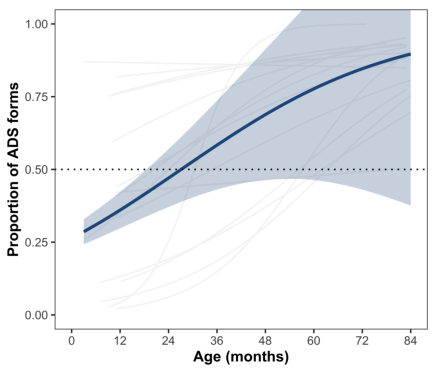
\includegraphics{figs/shift-timing-fig-1} 

}

\caption[Model-predicted increase in production of ADS forms with age]{Model-predicted increase in production of ADS forms with age. Gray lines depict raw individual word-pair trajectories.}\label{fig:shift-timing-fig}
\end{figure}
\end{CodeChunk}

Analyses of individual word-pair trajectories revealed significant
increases in production of ADS forms with age for 13 of 15 pairs.
Exploratory analyses of item effects also yielded evidence for three
distinct shift trajectory types (Figure 2). For some pairs (e.g.,
\emph{birdie/bird}), ADS forms dominated in children's speech from the
earliest ages sampled. For other pairs, CDS forms were initially more
prominent and were then replaced by ADS forms early on (e.g.,
\emph{doggy/dog} and \emph{night-night/goodnight} by 24 to 36 months) or
later in development (e.g., \emph{bunny/rabbit} and \emph{tummy/stomach}
after 48 months).

\begin{CodeChunk}
\begin{figure}[!ht]

{\centering 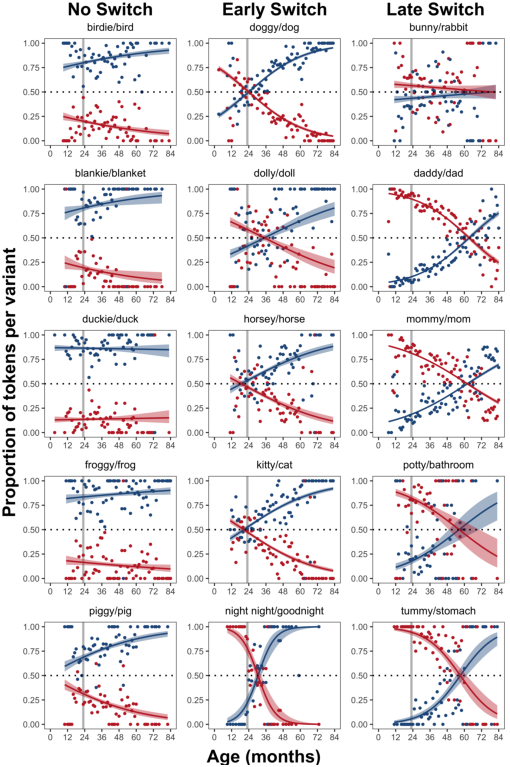
\includegraphics{figs/shift-timing-bypair-fig-1} 

}

\caption[Inidividual word-pair trajectories for increasing production of ADS forms (blue) and descreasing production of CDS forms (red) with age]{Inidividual word-pair trajectories for increasing production of ADS forms (blue) and descreasing production of CDS forms (red) with age. Columns indicate categorically different shift trajectory types: (1) items for which ADS forms appear to dominate in children's speech from the start, (2) items whose CDS forms are replaced by ADS forms early on, and (3) items whose ADS forms become dominant later in development.}\label{fig:shift-timing-bypair-fig}
\end{figure}
\end{CodeChunk}

\hypertarget{characterizing-the-input-in-what-linguistic-contexts-do-children-hear-cds-vs.-ads-forms}{%
\subsection{Characterizing the input: In what linguistic contexts do
children hear CDS vs.~ADS
forms?}\label{characterizing-the-input-in-what-linguistic-contexts-do-children-hear-cds-vs.-ads-forms}}

We used mixed-effects binomial logistic regression models to predict the
appearance of CDS vs.~ADS forms in given utterance on the basis of
target child's age, several linguistic properties of the utterance, and
interactions between each property and age. Models included random
slopes and intercepts for individual word pairs and speakers and were
fitted to all utterance data from speakers other than the target child.

Main effects and interactions with age are shown in Figure 2.

\begin{CodeChunk}
\begin{figure}[h]

{\centering 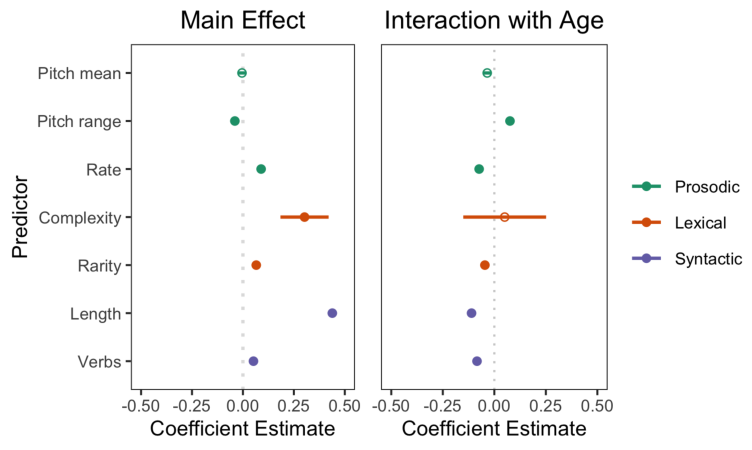
\includegraphics{figs/model-plot-1} 

}

\caption[Coefficient estimates for linguistic predictors of form]{Coefficient estimates for linguistic predictors of form. Positive main effects indicate that utterances are more likely to contain ADS forms when they have higher values for the predictor (e.g., faster speech rates). Positive age interactions indicate an increasing effect of the predictor with age. Error bars depict standard errors of the coefficient estimates, and filled circles represent significant effects (\textit{p} $<$ 0.05).}\label{fig:model-plot}
\end{figure}
\end{CodeChunk}

\hypertarget{modeling-learning-what-linguistic-information-is-most-useful-for-distinguishing-cds-vs.-ads-contexts}{%
\subsection{Modeling learning: What linguistic information is most
useful for distinguishing CDS vs.~ADS
contexts?}\label{modeling-learning-what-linguistic-information-is-most-useful-for-distinguishing-cds-vs.-ads-contexts}}

\hypertarget{discussion}{%
\section{Discussion}\label{discussion}}

\hypertarget{references}{%
\section{References}\label{references}}

\setlength{\parindent}{-0.1in} 
\setlength{\leftskip}{0.125in}

\noindent

\hypertarget{refs}{}
\begin{CSLReferences}{1}{0}
\leavevmode\hypertarget{ref-bergelsoncorpus}{}%
Bergelson, E. (2016). Bergelson HomeBank corpus.
\url{https://doi.org/10.21415/T5PK6D}.

\leavevmode\hypertarget{ref-boersma2016praat}{}%
Boersma, P., \& Weenink, D. (2016). Praat software. \emph{Amsterdam:
University of Amsterdam}.

\leavevmode\hypertarget{ref-braginsky2021childesr}{}%
Braginsky, M., Sanchez, A., \& Yurovsky, D. (2021). \emph{Childesr:
Accessing the 'CHILDES' database}. Retrieved from
\url{https://CRAN.R-project.org/package=childesr}

\leavevmode\hypertarget{ref-cooper1990preference}{}%
Cooper, R. P., \& Aslin, R. N. (1990). Preference for infant-directed
speech in the first month after birth. \emph{Child Development},
\emph{61}(5), 1584--1595.

\leavevmode\hypertarget{ref-fenson1994variability}{}%
Fenson, L., Dale, P. S., Reznick, J. S., Bates, E., Thal, D. J.,
Pethick, S. J., \ldots{} Stiles, J. (1994). Variability in early
communicative development. \emph{Monographs of the Society for Research
in Child Development}, i--185.

\leavevmode\hypertarget{ref-fernald1989intonation}{}%
Fernald, A. (1989). Intonation and communicative intent in mothers'
speech to infants: Is the melody the message? \emph{Child Development},
1497--1510.

\leavevmode\hypertarget{ref-foushee2016lexical}{}%
Foushee, R., Griffiths, T., \& Srinivasan, M. (2016). Lexical complexity
of child-directed and overheard speech: Implications for learning. In
\emph{Proceedings of the 38th annual conference of the cognitive science
society} (pp. 1697--1702).

\leavevmode\hypertarget{ref-frank2017wordbank}{}%
Frank, M. C., Braginsky, M., Yurovsky, D., \& Marchman, V. A. (2017).
Wordbank: An open repository for developmental vocabulary data.
\emph{Journal of Child Language}, \emph{44}(3), 677--694.

\leavevmode\hypertarget{ref-golinkoff2015baby}{}%
Golinkoff, R. M., Can, D. D., Soderstrom, M., \& Hirsh-Pasek, K. (2015).
(Baby) talk to me: The social context of infant-directed speech and its
effects on early language acquisition. \emph{Current Directions in
Psychological Science}, \emph{24}(5), 339--344.

\leavevmode\hypertarget{ref-honnibal2020spacy}{}%
Honnibal, M., Montani, I., Van Landeghem, S., \& Boyd, A. (2020).
{spaCy: Industrial-strength Natural Language Processing in Python}.
http://doi.org/\href{https://doi.org/10.5281/zenodo.1212303}{10.5281/zenodo.1212303}

\leavevmode\hypertarget{ref-kidd2012goldilocks}{}%
Kidd, C., Piantadosi, S. T., \& Aslin, R. N. (2012). The goldilocks
effect: Human infants allocate attention to visual sequences that are
neither too simple nor too complex. \emph{PloS One}, \emph{7}(5),
e36399.

\leavevmode\hypertarget{ref-macwhinney2000childes}{}%
MacWhinney, B. (2000). \emph{The CHILDES project: The database} (Vol.
2). Psychology Press.

\leavevmode\hypertarget{ref-manybabies2020quantifying}{}%
ManyBabies, C. (2020). Quantifying sources of variability in infancy
research using the infant-directed-speech preference. \emph{Advances in
Methods and Practices in Psychological Science}, \emph{3}(1), 24--52.

\leavevmode\hypertarget{ref-soderstromcorpus}{}%
McDivitt, K., \& Soderstrom, M. (2016). McDivitt HomeBank corpus.
\url{https://doi.org/10.21415/T5KK6G}.

\leavevmode\hypertarget{ref-nencheva2021moment}{}%
Nencheva, M. L., Piazza, E. A., \& Lew-Williams, C. (2021). The
moment-to-moment pitch dynamics of child-directed speech shape toddlers'
attention and learning. \emph{Developmental Science}, \emph{24}(1),
e12997.

\leavevmode\hypertarget{ref-rowe2008child}{}%
Rowe, M. L. (2008). Child-directed speech: Relation to socioeconomic
status, knowledge of child development and child vocabulary skill.
\emph{Journal of Child Language}, \emph{35}(1), 185--205.

\leavevmode\hypertarget{ref-shneidman2012language}{}%
Shneidman, L. A., \& Goldin-Meadow, S. (2012). Language input and
acquisition in a mayan village: How important is directed speech?
\emph{Developmental Science}, \emph{15}(5), 659--673.

\leavevmode\hypertarget{ref-soderstrom2007beyond}{}%
Soderstrom, M. (2007). Beyond babytalk: Re-evaluating the nature and
content of speech input to preverbal infants. \emph{Developmental
Review}, \emph{27}(4), 501--532.

\leavevmode\hypertarget{ref-vandamcorpus}{}%
VanDam, M. (2016). VanDam2 HomeBank corpus.

\leavevmode\hypertarget{ref-homebank}{}%
VanDam, M., Warlaumont, A. S., Bergelson, E., Cristia, A., De Palma, P.,
\& MacWhinney, B. (2016). Homebank: An online repository of daylong
child-centered audio recordings. \url{https://homebank.talkbank.org}.

\leavevmode\hypertarget{ref-vosoughi2012longitudinal}{}%
Vosoughi, S., \& Roy, D. K. (2012). A longitudinal study of prosodic
exaggeration in child-directed speech.

\leavevmode\hypertarget{ref-warlaumontcorpus}{}%
Warlaumont, A. S., \& Pretzer, G. M. (2016). Warlaumont HomeBank corpus.
\url{https://doi.org/10.21415/t54s3c}.

\leavevmode\hypertarget{ref-weisleder2013talking}{}%
Weisleder, A., \& Fernald, A. (2013). Talking to children matters: Early
language experience strengthens processing and builds vocabulary.
\emph{Psychological Science}, \emph{24}(11), 2143--2152.

\end{CSLReferences}

\bibliographystyle{apacite}


\end{document}
